\chapter{Introducción}
En este capítulo analizaremos algunos ejemplos de iteraciones de funciones
racionales. El objetivo es desarrollar una intuición sobre los fenómenos que
estudia la Dinámica Compleja y formalizar algunos conceptos básicos que
encontraremos en los ejemplos. Para ello, trabajaremos en el plano complejo
extendido (o esfera de Riemann) $\ExtC = \C \cup \{\infty\}$.

% --- SECCIÓN ------------------------------------------------------------------
% --- TRANSFORMACIONES DE MÖBIUS -----------------------------------------------
\section{Transformaciones de Möbius}
Comencemos con el caso más sencillo: las funciones racionales de grado uno.
Estas funciones, conocidas como transformaciones de Möbius, poseen una dinámica
sencilla de analizar.

\begin{definicion}[Función racional]
    Una \emph{función racional} es una función $R: \ExtC \to \ExtC$ de la forma
    \begin{equation*}
        R(z) = \frac{P(z)}{Q(z)},
    \end{equation*}
    donde $P(z)$ y $Q(z)$ son polinomios, sin ser ambos el polinomio nulo.
\end{definicion}

Supongamos que ni $P$ ni $Q$ son el polinomio nulo, en este caso $R$ no está
definido en las raíces comunes de $P$ y $Q$. Sin embargo, si estas existen,
podemos cancelar los factores comunes de $P$ y $Q$, obteniendo así dos
polinomios que no tendrán raíces comunes $P_1$ y $Q_1$. De ahora en adelante
consideraremos $P$ y $Q$ no tienen raíces comunes, y si las tuvieran,
consideraríamos $R = P_1/Q_1$. En estas circunstancias seguiremos los convenios
habituales con el punto del infinito en la esfera de Riemann: si $Q$ es el
polinomio nulo, entonces $R$ es la función constante $\infty$; si $Q(z) = 0$ y
$P$ no es el polinomio nulo, entonces $R(z) = \infty$; y tomaremos $R(\infty) =
\lim_{z \to \infty} R(z)$.

La preguntas fundamentales que nos hacemos son: si iteramos una función racional
$R$ partiendo de un punto arbitrario $z_0 \in \ExtC$, ¿cómo se comportará la
secuencia $R^n(z_0)$?; y si tomamos otro punto $w_0 \in \ExtC$ cercano a $z_0$,
¿$R^n(w_0)$ se comportará de manera similar a $R^n(z_0)$? A lo largo de todo el
trabajo se utilizará $R$ para referirse a una función racional y $R^n$ para
referirse a componer $R$ consigo misma $n$ veces.

Con fin de responder a la primera pregunta, necesitaremos introducir los
siguientes conceptos básicos.

Dada una función $g$ de un conjunto $X$ a sí mismo
($g: X \to X$), y dados $x$ e $y$ dos puntos en $X$, definimos la relación
$\sim$ en $X$ de la siguiente manera: $x \sim y$ si y solo si existen $n$ y $m$
enteros tales que
\begin{equation*}
    g^n(x) = g^m(y).
\end{equation*}
Se puede comprobar que la relación $\sim$ es reflexiva, simétrica y transitiva
y, por tanto, es una relación de equivalencia.

\begin{definicion}[Órbita, órbita positiva y órbita negativa de $x$]
    En estas circunstancias, llamaremos \emph{órbita} de $x$ a la clase de
    equivalencia dicho punto, y la denotaremos por $[x]$. Además, definiremos la
    órbita positiva de $x$ cómo el conjunto
    \begin{equation*}
        \orbit^+(z) = \{R^n(z) \mid n \geq 1\};
    \end{equation*}
    y órbita negativa al conjunto
    \begin{align*}
        \orbit^-(z) &= \{w \mid \exists n \geq 0 \text{ tal que } R^n(w) = z\} \\
                    &= \bigcup_{n \geq 0} R^{-n}\{z\},
    \end{align*}
\end{definicion}

\begin{definicion}[Punto fijo]
    Sea $D$ un conjunto y $f \colon D \to \ExtC$ una función racional. Un punto
    $\zeta \in D$ diremos que es un \emph{punto fijo} de $f$ si $f(\zeta) =
    \zeta$.
\end{definicion}

\begin{definicion}[Transformación de Möbius]
    Una transformación de Möbius es una función racional de la forma
    \[
        R(z) = \frac{az+b}{cz+d}, \quad ad-bc \ne 0
    \] 
    donde $z$, $a$, $b$, $c$, $d$ son números complejos.
\end{definicion}

Siguiendo los convenios habituales con el punto del infinito en la esfera de
Riemann: $R(\infty)=a/c$ y $R(-d/c) = \infty$.

Ahora, usando las transformaciones de Möbius, veremos con ejemplos en que se
traducen estos conceptos. Pero, antes resulta interesante introducir el concepto
de \emph{conjugación}. No solo nos va a servir para simplificar el análisis de
las transformaciones de Möbius, sino que también nos ayudará a encontrar
familias de funciones con el mismo comportamiento dinámico por ser una relación
de equivalencia.

\begin{definicion}[Conjugación]
    Sean $X$, $Y \subseteq \ExtC$, $R \colon X \to X$ y $S \colon Y \to Y$ dos
    funciones racionales. Decimos que $R$ y $S$ son conjugadas si existe una
    transformación de Möbius $g \colon X \to Y$ tal que
    \[
        R = g^{-1} S g.
    \]
\end{definicion}

Su utilidad en el análisis de la dinámica radica en que al iterar $R$, los
términos intermedios $g$ y $g^{-1}$ se cancelan, obteniendo
\[
    R^n = (g^{-1} S g) (g^{-1} S g) \dots (g^{-1} S g) = g^{-1} S^n g.
\]
Por tanto, estudiar las órbitas de $R$ es equivalente a estudiar las de $S$. Los
puntos fijos y periódicos, y la convergencia de las órbitas se preservan bajo la
aplicación de $g$.

\begin{ejemplo}
    Consideremos como primer ejemplo la transformación
    \begin{equation}\label{eq:mobius_ej1}
        R(z) = \frac{3z-2}{2z-1}.
    \end{equation}
    Esta función tiene un único punto fijo, $\zeta = 1$. Utilizando $g =
    1/(z-\zeta)$ para trasladar el punto fijo $\zeta$ al infinito, encontramos
    que $R$ es conjugada a $S(z) = 2 + z$. $S$ es una traslación y $S^n(z) = 2n
    + z$. Observamos que el único punto fijo de $S$ es el infinito (que se
    corresponde con el punto fijo $\zeta = 1$ de $R$) y que dado cualquier punto
    $z_0 \in \ExtC$, $S^n(z_0)$ tiene al punto fijo cuando $n \to \infty$.
    Luego, $\lim_{n \to \infty} R^n(z_0) = \zeta$ para todo $z_0 \in \ExtC$.
\end{ejemplo}

\begin{observacion}
    En general, sea $R$ una transformación de Möbius con un único punto fijo.
    Entonces, $R$ es conjugada a una traslación y $\lim_{n \to \infty} R^n(z_0)
    = \zeta$ para todo $z_0 \in \ExtC$. Puede verse una demostración en
    \cite[4-5]{Beardon1991}.
\end{observacion}

\begin{ejemplo}
    Veamos ahora un escenario distinto con la transformación
    \[
        R(z) = \frac{(1+i)z + (1-i)}{(1-i)z + (1+i)},
    \]
    la cual posee dos puntos fijos, $\zeta_1 = 1$ y $\zeta_2 = -1$. Esta vez
    usamos $g(z) = (z-\zeta_2)/(z-\zeta_1)$ para enviar los puntos fijos $1$ y
    $-1$ al $\infty$ y al $0$ respectivamente. Obtenemos que $R$ es conjugada a
    la rotación $S(z) = iz$. Como $(-i)^4=1$, se tiene que $S^4(z)=z$ para todo
    $z$ y, en consecuencia por las propiedades de la conjugación, $R^4(z)= z$.
    Bajo esta transformación, todas las órbitas son periódicas (de período
    divisor de 4) y, salvo en los puntos fijos, ninguna órbita converge.
\end{ejemplo}

\begin{observacion}
    En general, sea $R$ una transformación de Möbius con dos puntos fijos.
    Entonces, $R$ es conjugada a una función de la forma $S(z) = az$, con $a \in
    \ExtC$, y se da uno de los siguientes casos para todo $z_0 \in \ExtC$:
    \begin{enumerate}
        \item $R^n(z_0)$ converge a uno de los puntos fijos (si $|a| \neq 1$);
        \item $z_0$ es un punto periódico;
        \item o $\mathcal{O}(z_0)$ forma un subconjunto denso de una
        circunferencia o recta.
    \end{enumerate}
    Puede verse una demostración en \cite[5]{Beardon1991}.
\end{observacion}

En las transformaciones de Möbius, dados dos puntos cercanos cualesquiera $z_0$
y $w_0 \in \ExtC$, ambos describirán órbitas prácticamente iguales.


% --- SECCIÓN ------------------------------------------------------------------
% --- LA FAMILIA CUADRÁtica ----------------------------------------------------
\section{La familia cuadrática: $z^2 + c$}
Al incrementar el grado a dos, la aparente simplicidad desaparece rápidamente.
Empecemos examinando el polinomio cuadrático más elemental:
\[
    P(z) = z^2.
\]
Sus puntos fijos son $0$, $1$, e infinito. Es inmediato comprobar que si
partimos de un punto en el disco unidad abierto ($|z| < 1$), su órbita tiende a
$0$. Por el contrario, si partimos del exterior del disco ($|z| > 1$), su órbita
escapa a $\infty$.% (Figura~\ref{fig:z_squared_fatou_basins_and_times}).

% \begin{figure}[htbp] \centering
%     
\includegraphics[width=0.5\textwidth]{z_squared_fatou_basins_and_times.pdf}
%     \caption{Plano dinámico de $P(z)=z^2$. En rojo se ve el subconjunto de
%     $\ExtC$ que converge a $0$, y en azul el que converge a $\infty$. Cuanto
%     más oscuro es el color de un punto más rápido converge. La frontera en
%     blanco que separa ambas cuencas es la circunferencia unidad.}
%     \label{fig:z_squared_fatou_basins_and_times} \end{figure}

Pero, ¿qué ocurre en la frontera que separa ambas cuencas, es decir, en la
circunferencia unidad $C = \{z \colon |z| = 1\}$? Dado que $|z^2| = 1 \iff |z| =
1$, sabemos que para cada $z_0 \in C$, $\mathcal{O}^+(z_0) \subseteq C$ y
$\mathcal{O}^-(z_0) \subseteq C $. Diremos que $C$ es un conjunto
\emph{completamente invariante}.

\begin{definicion}[Conjunto invariante]
    Dados un conjunto $X$ y una función $g \colon X \to X$, un subconjunto $E
    \subseteq X$ es:
    \begin{enumerate}
        \item \emph{positivamente invariante} si $g(E) = E$;
        \item \emph{negativamente invariante} si $g^{-1}(E) = E$;
        \item \emph{completamente invariante} si $g(E) = E = g^{-1}(E)$.
    \end{enumerate}
\end{definicion}

Dentro de $C$, la dinámica de $R(z)=z^2$ (que sobre esta curva equivale a
duplicar el ángulo, $\theta \mapsto 2\theta \pmod{2\pi}$) es caótica.
Dependiendo del punto inicial $z_0 \in C$, podemos encontrar órbitas que
convergen a $1$ en tiempo finito (las correspondientes a ángulos de la forma
$2\pi r / 2^m$), órbitas periódicas de cualquier periodo, e incluso órbitas
densas en $C$ \cite[6--8]{Beardon1991}. 

Esta sensibilidad a las condiciones iniciales marca una diferencia clara con las
transformaciones de Möbius: dos puntos arbitrariamente cercanos en $\ExtC$ (uno
en $C$, otro ligeramente fuera) tendrán futuros radicalmente distintos.

\subsection{Fractales}
Además de simplificar el cálculo de órbitas, la conjugación nos permite reducir
y clasificar familias enteras de funciones. Un ejemplo de esto ocurre en grado
dos. Un polinomio cuadrático general tiene la forma $P(z) = az^2 + bz + d$,
dependiendo de tres parámetros complejos: $a$, $b$, $d \in \C$. Sin embargo,
mediante una conjugación podemos transformar cualquier polinomio de grado dos a
uno de la forma
\[
    P_c(z) = z^2 + c, \quad c \in \C,
\]
eliminando así dos coeficientes. Esta familia de un solo parámetro encierra toda
la complejidad dinámica de los polinomios de grado dos.

En los polinomios, debido a que para el punto del infinito es siempre un punto
fijo atractor, podemos dividir el plano complejo en dos regiones con
comportamientos cualitativamente opuestos: los puntos que son arrastrados al
infinito y los que permanecen acotados. La frontera entre estas regiones será el
epicentro del comportamiento caótico: dado un punto inicial $z_0$ en la
frontera, variaciones infinitesimales en el punto inicial alterarán el destino
de la órbita por completo.

En caso analizado $P_0(z) = z^2$ esta frontera se correspondía con la
circunferencia unidad. Sin embargo, tomando otros valores de $c$ diferentes
podemos observar, con ayuda de un ordenador, conjuntos cuyas fronteras no son
curvas suaves como la circunferencia del caso $c=0$, sino que presentan una
estructura fractal (Figura~\ref{fig:z_squared_plus_c_escape_times}).

\begin{figure}[htbp]
    \centering
    % Top Row
    \begin{subfigure}[b]{0.48\textwidth}
        \centering
        
\includegraphics[width=\textwidth]{z_squared_minus_one_escape_times.pdf}
        \caption{$c = -1$.}
        \label{fig:z_squared_minus_one_escape_times}
    \end{subfigure}
    %\hfill % Adds horizontal space between the two images
    \begin{subfigure}[b]{0.48\textwidth}
        \centering
        
\includegraphics[width=\textwidth]{z_squared_plus_c5_escape_times.pdf} 
        \caption{$c = -0.122... - 0.744...\, i$.}
        \label{fig:z_squared_plus_c5_escape_times}
    \end{subfigure}

    %\vspace{0.5cm} % Adds vertical space between the rows

    % Bottom Row
    \begin{subfigure}[b]{0.48\textwidth}
        \centering
        
\includegraphics[width=\textwidth]{z_squared_plus_c1_escape_times.pdf}
        \caption{$c = -0.836 - 0.232i$.}
        \label{fig:z_squared_plus_c1_escape_times}
    \end{subfigure}
    %\hfill
    \begin{subfigure}[b]{0.48\textwidth}
        \centering
        
\includegraphics[width=\textwidth]{z_squared_plus_c2_escape_times.pdf}
        \caption{$c = 0.285 + 0.01i$.}
        \label{fig:z_squared_plus_c2_escape_times}
    \end{subfigure}

    % Main Caption
    \caption{Diferentes planos dinámicos para polinomios de la familia
    cuadrática $P_c(z) = z^2 + c$. La región en negro son los puntos que no
    escapan a infinito bajo la iteración de $P_c$. El resto de puntos, cuanto
    más claro es el color, más rápido divergen a infinito.}
    \label{fig:z_squared_plus_c_escape_times}
\end{figure}

Dependiendo del valor de $c$, las regiones que permanecen acotadas pueden
deformarse, fragmentarse o incluso desaparecer, dando lugar a la famosa
dicotomía topológica que define el conjunto de Mandelbrot
(Figura~\ref{fig:mandelbrot_set}): la frontera donde reside la dinámica caótica
puede ser un conjunto conexo (como para $c=0$ y $c=-1$) o una nube de puntos
totalmente no conexa (como para $c=1$).

\begin{figure}[htbp]
    \centering
    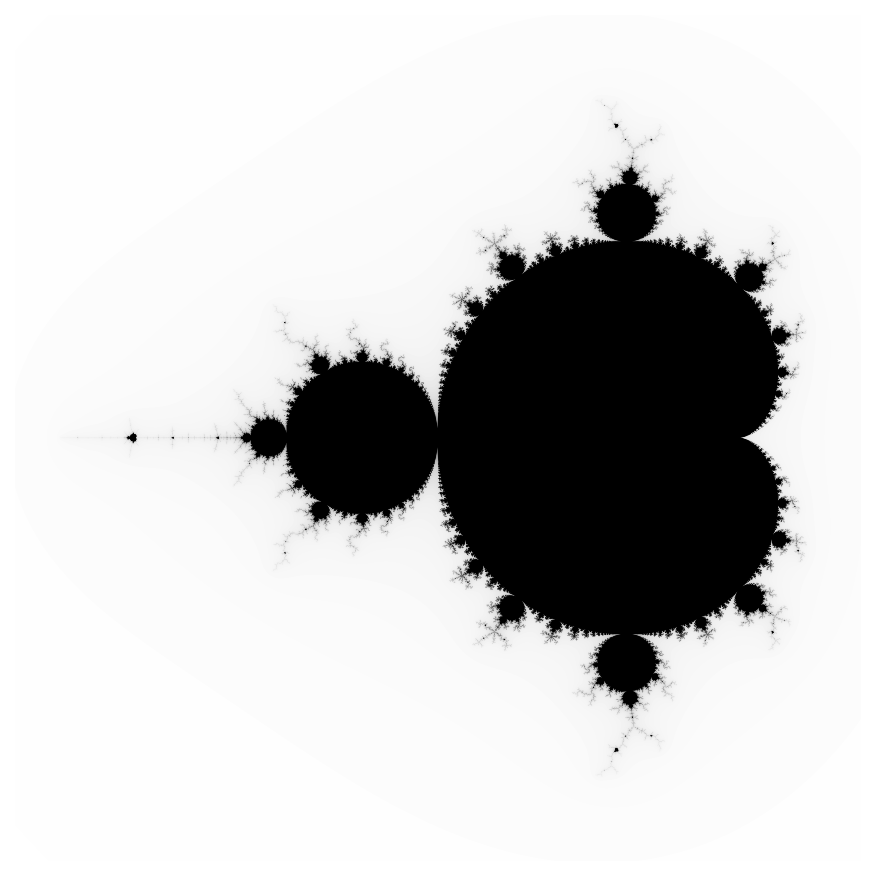
\includegraphics[width=0.5\textwidth]{../figures/mandelbrot_set.pdf}
    \caption{El conjunto de Mandelbrot. En negro los valores de $c$ para los
    cuales la frontera donde reside la dinámica compleja de $P_c$ es conexa.}
    \label{fig:mandelbrot_set}
\end{figure}

% --- SECCIÓN ------------------------------------------------------------------
% --- EL MÉTODO DE NEWTON ------------------------------------------------------
\section{El método de Newton}
Los ejemplos anteriores surgen de iterar funciones por el mero interés de
estudiar su dinámica. Sin embargo, los sistemas dinámicos complejos también
aparecen de forma natural en problemas numéricos prácticos, siendo el caso más
paradigmático la búsqueda de raíces de un polinomio $P(z)$ mediante el método de
Newton-Raphson extendido al plano complejo.

Este método consiste en la iteración de la función de Newton asociada a $P(z)$,
la cual constituye siempre una función racional:
\[
    N_P(z) = z - \frac{P(z)}{P'(z)}.
\]
Es inmediato comprobar que los puntos fijos finitos de $N_P(z)$ coinciden
exactamente con las raíces de $P(z)$. Además, un resultado clásico de
convergencia local asegura que si la condición inicial $z_0$ se escoge
suficientemente cerca de una de estas raíces, la sucesión de iterados convergerá
a ella (véase, por ejemplo, \cite{Beardon1991}).

Determinar globalmente qué regiones del plano convergen a cada raíz resultó ser
una tarea compleja. Este problema fue planteado originalmente por Cayley en 1879
en un artículo de la \emph{American Mathematical Society} \cite{Cayley1879} al
estudiar la extensión del algoritmo al plano complejo.

Para polinomios cuadráticos, como $P(z) = z^2 - 1$, el comportamiento global es
el esperado. El plano complejo se divide simétricamente en dos regiones de
convergencia. La frontera es la recta mediatriz de las raíces, y los puntos de
esta dan lugar a órbitas que jamás convergen
(Figura~\ref{fig:z_squared_minus_one_newton_fatou_basins_and_times}).

Sin embargo, al incrementar el grado del polinomio a tres, como en $P(z) = z^3 -
1$, la simplicidad global desaparece. La frontera que separa las regiones de
convergencia hacia cada una de las tres raíces deja de ser una línea sencilla y
se transforma en un conjunto infinitamente intrincado y fractal
(Figura~\ref{fig:z_cubed_minus_one_newton_fatou_basins_and_times}).

\begin{figure}[htbp]
    \centering
    % Top Row
    \begin{subfigure}[b]{0.48\textwidth}
        \centering
        
\includegraphics[width=\textwidth]{z_squared_minus_one_newton_fatou_basins_and_times.pdf}
        \caption{$P(z) = z^2 -1$.}
        \label{fig:z_squared_minus_one_newton_fatou_basins_and_times}
    \end{subfigure}
    \hfill % Adds horizontal space between the two images
    \begin{subfigure}[b]{0.48\textwidth}
        \centering
        
\includegraphics[width=\textwidth]{z_cubed_minus_one_newton_fatou_basins_and_times.pdf} 
        \caption{$P(z) = z^3 - 1$.}
        \label{fig:z_cubed_minus_one_newton_fatou_basins_and_times}
    \end{subfigure}

    % Main Caption
    \caption{Planos dinámicos de $N_P(z)$. Cada color representa el conjunto de
    puntos que convergen a una misma raíz de $P$ (cuantas más oscuros, mayor
    velocidad de convergencia).}
    \label{fig:newton_fatou_basins_and_times}
\end{figure}

Esta división fractal del plano es una muestra más de cómo la iteración de
funciones racionales separa de forma natural la esfera de Riemann en dos
regiones cualitativamente opuestas: una donde la dinámica es estable (las zonas
de convergencia) y otra donde el comportamiento es inestable y de gran
complejidad topológica (las fronteras). Formalizar estas dos regiones, conocidas
como el conjunto de Fatou y el conjunto de Julia, será el objetivo central del
próximo capítulo.